\documentclass[../../rapport.tex]{subfiles}

\begin{document}
  Pour construire un nouveau type à partir d'autres, on doit donner 3 règles :
  \begin{itemize}
    \item \textbf{Formation du type}, qui permet de construire un type à partir d'autres types ou famille de types,
    \item \textbf{Introduction}, qui explique comment sont construits les éléments de ce type,
    \item \textbf{Élimination}, décrivant comment utiliser ces éléments.
  \end{itemize}

  Partant de ces 3 règles, on peut construire un type et éventuellement ajouter des règles supplémentaires concernant
  leur comportement par rapport à l'égalité par définition.

  \subsubsection{Univers}

  Plus tôt, on a utilisé un jugement de la forme "$\Gamma \vdash A\ \text{type}$" pour signifier que $A$ est un type.
  Cependant ce jugement n'est pas un jugement de la théorie, on se ramène alors à un autre jugement déjà présent :
  le jugement de typage.
  Pour ce faire, on doit introduire un type composé de type, un type univers $\U$.
  Pour la même raison, on voudrais dire que $\U$ est lui-même un élément d'un type plus grand et ainsi de suite.
  Pour résoudre ce problème, on postule qu'il existe une hiérarchie de type
  $$\U_0,\ \U_1,\ \U_2,\ \hdots,\ \U_i,\ \hdots$$
  telle que $\U_i : \U_{i+1}$.

  Pour ces types, on a seulement une règle d'introduction et une règle décrivant la hiérarchie entre ces types :

  $$
  \begin{array}{cc}
    \prftree[r]{($\U$ i)}{\Gamma \ctx}{\Gamma \vdash U_i : U_{i+1}} \hspace{2cm}
    & \prftree[r]{($\U$ cumul)}{\Gamma \vdash A : \U_i}{\Gamma \vdash A : \U_{i+1}}
  \end{array}
  $$

  Par conséquent, la règle sur les contextes devient la suivante :

  $$
  \prftree[r]{($\ctx$)}{(a_1 : A_1, \hdots, a_{n-1} : A_{n-1}) \vdash A_n : \U_k}
    {(a_1 : A_1, \hdots, a_n : A_n) \ctx}
  $$

  \subsubsection{Fonctions}

  Étant donné deux types $A, B : \U$, on peut former le type des fonctions de $A$ dans $B$ noté $A \fun B$
  grâce à la règle de formation suivante :

  $$
  \prfinterspace=2em
  \prftree[r]{($\fun$ f)}{\Gamma \vdash A : \U_i}{\Gamma \vdash B : \U_i}{\Gamma \vdash A \fun B : \U_i}
  $$

  Une fonction est donc un élément $f$ de type $A \fun B$.
  Si on se donne $a : A$, on peut évaluer $f$ en $a$ ce qui donne un élément de type $B$
  que l'on note $f\ a$ ou bien $f(a)$ qui est appelé valeur de $f$ en $a$, c'est la règle d'élimination de $\fun$ :

  $$
  \prfinterspace=2em
  \prftree[r]{($\fun$ e)}{\Gamma \vdash f : A \fun B}{\Gamma \vdash a : A}{\Gamma \vdash f\ a : B}
  $$

  Pour former une fonction $f$ de $A$ dans $B$ \textit{ie.} un élément de type $A \fun B$,
  la manière canonique de faire est d'utiliser les $\lambda$-abstraction et la règle d'introduction suivante :

  $$
  \prftree[r]{($\fun$ i)}{\Gamma, x : A \vdash \Phi : B}{\Gamma \vdash \lambda (x : A). \Phi : A \fun B}
  $$
  Dans cette règle $\Phi$ correspond à une formule qui peut éventuellement faire intervenir la variable $x$.

  Enfin, lorsque l'on considère une fonction $f : A \fun B$ définie par $f :\equiv \lambda (x : A). \Phi$
  où $\Phi$ est une formule et un élément $a : A$, il est naturel que la valeur de $f$ en $a$ soit égale à
  la formule $\Phi$ où l'on remplace les occurences de $x$ par des $a$, ce que l'on note $\Phi[a/x]$.
  Ce comportement est en fait une règle d'égalité que l'on peut énoncer sous cette forme :

  $$
  \prfinterspace=2em
  \prftree[r]{($\beta$)}{\Gamma, x : A \vdash \Phi : B}{\Gamma \vdash a : A}
    {\Gamma \vdash (\lambda(x : A).\Phi)\ a \equiv \Phi[a/x]}
  $$

  \begin{example}
    Considérons un type $A : \U$ et la fonction "identité" de $A$ définie par $I :\equiv \lambda(x : A).x$.
    Pour prouver que le type de $I$ est bien $A \fun A$, on peut utiliser les règles énoncées précédemment :

    $$
    \prftree
      {\prftree
	{\prfaxiom{A : \U \vdash A : \U}}
	{A : \U, x : A \vdash x : A}}
      {A : \U \vdash \lambda(x : A). x : A \fun A}
    $$
  \end{example}

  On a vu jusqu'ici comment construire des fonctions à une variable, on peut alors généraliser pour obtenir
  des fonctions à plusieurs variables.
  Pour ce faire, considérons trois types $A, B, C : \U$.
  Naïvement, on voudrais construire une fonction de type $A \times B \fun C$,
  mais le type $A \times B$ n'est pas encore défini.
  Pour contourner ce problème, on peut voir une fonction $f$ de $A \times B \fun C$ comme

  \begin{align}
    f(x, y) = (\lambda(a : A). f(a, y)) x &= ((\lambda(a : A). (\lambda(b : B). f(a, b)))\ x)\ y \\ 
					  &= (\lambda(a : A).\lambda(b : B). f(a, b))\ x\ y.
  \end{align}

  On a ainsi obtenu une fonction de type $A \fun B \fun C$ qui prend les mêmes valeurs que $f$
  grâce à ce processus de \textit{curryfication}.

  \begin{example}
    Considérons deux types $A, B : \U$ et la fonction $K$ définie par
    $$K :\equiv \lambda(x : A).(\lambda(y : B).x)$$
    Grâce à un arbre similaire au précédent, on trouve que le type de $K$ est $A \fun B \fun A$
    (on omet les parenthèses en prenant comme convention que $A \fun A \fun A$ est égal à $A \fun (A \fun A)$).
    De plus, on peut également montrer que si $a : A$ et $b : B$, alors $K\ a\ b \equiv a$. En effet, \textsc{A faire.}
    % $$
    % \prfinterspace=2em
    % \prftree{}
    % $$
  \end{example}

  Si on considère deux types $A, B : \U$ et qu'on les voit comme des propositions,
  alors le type $A \fun B$ peut s'interpreter comme l'implication $A \implies B$.

  \subsubsection{Fonctions dépendantes ($\Pi$-type)}

  Une manière de généraliser le type des fonctions est de définir un type de fonctions dépendantes (ou $\prod$-type),
  qui est un type de fonction dont le codomaine dépend du point d'application de la fonction.

  Pour former ce nouveau type, on considère $A : \U$ un type et $B : A \fun \U$ une famille de type indexée sur $A$.
  On peut alors former le type $\prod_{a : A}{B(a)}$ grâce à la règle de formation suivante : \textsc{Revoir avec univers}

  $$
  \prfinterspace=2em
  \prftree[r]{($\Pi$ f)}{\Gamma \vdash A : \U_i}{\Gamma, a : A \vdash B(a) : \U_i}
    {\Gamma \vdash \prod_{a:A}{B(a)} : \U_i}
  $$

  On construit des éléments de type $\prod_{a:A}{B(a)}$ de manière analogue aux fonctions en utilisant des $\lambda$-abstractions.
  En effet, $\lambda(a : A). \Phi$ est de type $\prod_{a:A}{B(a)}$ si lorsque $a : A$, alors $\Phi : B(x)$.
  Cette règle énoncé plus formellement est la règle d'introduction de ce nouveau type :

  $$
  \prftree[r]{($\Pi$ i)}{\Gamma, a : A \vdash \Phi : B(a)}
    {\Gamma \vdash \lambda(a : A). \Phi : \prod_{a:A}{B(a)}}
  $$

  Ensuite, la règle d'élimination est similaire à celle des types de fonctions.
  Si on considère $f : \prod_{a:A}B(a)$ et $a : A$, alors $f\ a$ est de type $B(a)$,
  ce que l'on peut traduire avec la règle suivante :

  $$
  \prfinterspace=2em
  \prftree[r]{($\Pi$ e)}{\Gamma \vdash f : \prod_{a:A}{B(a)}}{\Gamma \vdash a : A}
    {\Gamma \vdash f\ a : B(a)}
  $$

  Également, la règle $\beta$ des fonctions se généralise au $\prod$-type :

  $$
  \prfinterspace=2em
  \prftree[r]{($\beta$)}{\Gamma, x : A \vdash \Phi : B(x)}{\Gamma \vdash a : A}
    {\Gamma \vdash (\lambda(x : A).\Phi)\ a \equiv \Phi[a/x]}
  $$

  L'utilité des types de fonctions dépendantes est notamment de pouvoir définir des fonctions de façon polymorphes,
  comme le montre les exemples suivants.

  \begin{example}
    La fonction identité du paragraphe précédent était défini sur un type $A : \U$ quelconque.
    On peut alors généraliser sa définition de la manière suivante :

    $$I \equiv \lambda (A : \U). \lambda (a : A).\ a : \prod_{A : \U}{A \fun A}.$$
    Ainsi définie, la fonction $I$ ne dépend pas d'un type préexistant.

    On peut également redéfinir la fonction constante $K$ d'une manière analogue :

    $$K \equiv \lambda (A : \U). \lambda (B : \U). \lambda (x : A). \lambda (y : B).\ x :
      \prod_{A : \U}\prod_{B : \U}{A \fun B \fun A}.$$

    Pour ces types et définition polymorphe, on peut également avoir la notation $I_A$ à la place de $I\ A$
    pour plus de clarté.
  \end{example}

  D'un autre point de vue ce type peut également être vu comme l'équivalent du $\forall$ de la logique
  du première ordre.
  En effet, si on considère $A : \U$ un type et $C : A \fun \U$ une famille de type,
  que l'on peut également voir comme un prédicat, alors le type $\prod_{a : A}{C(a)}$ se comporte comme
  la proposition $\forall a,\ C(a)$ en logique classique.

  \subsubsection{Type vide}

  On introduit le type vide $\0$, qui ne contient aucun élément et donc n'a pas de règle d'introduction mais seulement
  une régle de formation et d'élimination :

  $$
  \prfinterspace=2em
  \begin{array}{cc}
    \prftree[r]{($\0$ f)}{\Gamma \ctx}{\Gamma \vdash \0 : \U_i} \hspace{2cm}
    & \prftree[r]{($\0$ e)}{\Gamma \vdash C : \U_i}{\Gamma \vdash a : \0}{\Gamma \vdash \rec_{\0}(C, a) : C}
  \end{array}
  $$

  Ainsi, on a construit une fonction $\rec_{\0}$ de type $\prod_{C: \U} \0 \fun C$
  qui à un type $C : \U_i$ associe une fonction qui ne prend aucune valeur.
  Par conséquent, on ne devrais jamais calculer cette fonction,
  c'est la raison pour laquelle il n'y a pas de règle de calcul pour ce type.
  La règle d'élimination agit comme le principe \textit{ex falso quodlibet},
  en effet si on construit un élément du type vide (\textit{ie.} une preuve de $\bot$),
  alors on peut construire des éléments de n'importe quel type.

  \subsubsection{Type unité}

  Ensuite, dans l'objectif de construire tout les types finis, on commence par construire le type unité $\1$,
  contenant seulement un élément. Pour ce faire on a la règle de formation analogue à celle du type $\0$ avec
  une règle d'introduction simple car le type $\1$ ne possède qu'un seul élément :

  $$
  \prfinterspace=2em
  \begin{array}{cc}
    \prftree[r]{($\1$ f)}{\Gamma \ctx}{\Gamma \vdash \1 : \U_i} \hspace{2cm}
    & \prftree[r]{($\1$ i)}{\Gamma \ctx}{\Gamma \vdash \star : \1}
  \end{array}
  $$

  La règle d'élimination de $\1$ permet de construire des fonctions de $\1$ vers un autre type $C$,
  qui sont donc des fonctions constantes et c'est ce qu'affirme la règle de calcul du type unité.

  \begin{gather*}
    \prfinterspace=2em
    \prftree[r]{($\1$ e)}{\Gamma \vdash C : \U_i}{\Gamma \vdash c : C}{\Gamma \vdash p : \1}
      {\Gamma \vdash \rec_{\1}(C, p, c) : C} \\
    \prftree[r]{($\1 \equiv$)}{\Gamma \vdash C : \U_i}{\Gamma \vdash c : C}
      {\Gamma \vdash \rec_{\1}(C, \star, c) \equiv c : C}
  \end{gather*}
  où la fonction $\rec_{\1}$ est de type $\prod_{C : \U}\1 \fun C \fun C$
  (il est également possible d'intervertir les deux derniers arguments).

  De plus pour ce type, on a un principe d'unicité car le seul élément de $\1$ est $\star$ qui découle des règles précédentes.

  $$
  \prfinterspace=2em
  \prftree{
      \prftree{}
      {\Gamma \vdash \rec_{\1}(\1, p, \star) \equiv \star : \1}
    }
    {
      \Gamma \vdash p \equiv \rec_{\1}(\1, p, \star) : \1
    }
    {\Gamma \vdash p \equiv \star : \1}
  $$
  \textsc{A finir.}

  \subsubsection{Coproduit}

  Le dernier élément manquant pour construire tout les types finis sont les coproduits,
  qui permettent de construire un équivalent de l'union disjointe de la théorie des ensembles à partir de deux types
  comme l'exprime la règle de formation suivante :

  $$
  \prfinterspace=2em
  \prftree[r]{($+$ f)}{\Gamma \vdash A : \U_i}{\Gamma \vdash B : \U_i}
    {\Gamma \vdash A + B : \U_i}
  $$

  Étant donné deux types $A, B : \U_i$, un élément $e$ du type $A + B$ à deux manières d'être construit :
  \begin{itemize}
    \item soit $e$ est issu d'un élément $a : A$ et est donc de la forme $\inl(a)$,
    \item soit $e$ est issu d'un élément $b : B$ et est donc de la forme $\inr(b)$.
  \end{itemize}
  On a donc deux règles d'introduction pour les coproduits :

  $$
  \prfinterspace=1.2em
  \begin{array}{cc}
    \prftree[r]{($+ \inl)$}{\Gamma \vdash A : \U_i}{\Gamma \vdash B : \U_i}{\Gamma \vdash a : A}{\Gamma \vdash \inl(a) : A + B} \hspace{0.5cm}
    & \prftree[r]{($+ \inr)$}{\Gamma \vdash A : \U_i}{\Gamma \vdash B : \U_i}{\Gamma \vdash b : B}{\Gamma \vdash \inr(b) : A + B}
  \end{array}
  $$

  Pour prouver des propositions sur des coproduits, une manière naturelle de faire est de raisonner par cas :
  ou bien on a un élément de $A$ ou bien il s'agit d'un élément de $B$.
  Pour décrire cette méthode de raisonnement, on a la règle d'élimination des coproduits pour deux types $A, B : \U_i$ :

  $$
  \prfinterspace=1.2em
  \prftree[r]{($+$ e)}{\Gamma \vdash C : \U_i}{\Gamma, a : A \vdash g_0\ a : C}{\Gamma, b : B \vdash g_1\ b : C}{\Gamma \vdash e : A + B}
    {\Gamma \vdash \rec_{A+B}(C, g_0, g_1, e) : C}
  $$
  Ainsi, la fonction $\rec_{A+B}$ est de type $\prod_{C : \U}(A \fun C) \fun (B \fun C) \fun A + B \fun C$,
  et permet de faire la disjonction de cas.
  On a de plus deux règles décrivant le comportement de la fonction $\rec_{A+B}$ en fonction de son dernier argument :

  $$
  \prfinterspace=1.2em
  \prftree[r]{($+ \equiv_1$)}{\Gamma \vdash C : \U_i}{\Gamma, a : A \vdash g_0\ a : C}{\Gamma, b : B \vdash g_1\ b : C}{\Gamma \vdash x : A}
    {\Gamma \vdash \rec_{A+B}(C, g_0, g_1, \inl(x)) \equiv g_0\ x : C}
  $$

  $$
  \prfinterspace=1.2em
  \prftree[r]{($+ \equiv_2$)}{\Gamma \vdash C : \U_i}{\Gamma, a : A \vdash g_0\ a : C}{\Gamma, b : B \vdash g_1\ b : C}{\Gamma \vdash y : B}
    {\Gamma \vdash \rec_{A+B}(C, g_0, g_1, \inr(y)) \equiv g_1\ y : C}
  $$

  \begin{example}[Le type $\2$]
    Avec le coproduit et le type $\1$ on peut désormais construire le type $\2$ a deux éléments.
    En effet, on définit $\2$ par $\2 :\equiv \1 + \1$, ce qui donne la règle de formation
    $$
    \prfinterspace=1.2em
    \prftree{\prftree{\Gamma \ctx}{\Gamma \vdash \1 : \U_i}}{\prftree{\Gamma \ctx}{\Gamma \vdash \1 : \U_i}}
      {\Gamma \vdash \1 + \1 : \U_i}
    $$
    que l'on peut résumer à :
    $$
    \prftree[r]{($\2$ f)}{\Gamma \ctx}{\Gamma \vdash \2 : \U_i}
    $$

    Ensuite, comme pour le coproduit on a deux règles d'introduction :
    $$
    \prfinterspace=1.2em
    \begin{array}{cc}
      \prftree{\prftree{\Gamma \ctx}{\Gamma \vdash \1 : \U_i}}
	{\prftree{\Gamma \ctx}{\Gamma \vdash \1 : \U_i}}
	{\prftree{\Gamma \ctx}{\Gamma \vdash \star : \1}}
	{\Gamma \vdash \inl(\star) : \2} \hspace{1cm}
      &\prftree{\prftree{\Gamma \ctx}{\Gamma \vdash \1 : \U_i}}
	{\prftree{\Gamma \ctx}{\Gamma \vdash \1 : \U_i}}
	{\prftree{\Gamma \ctx}{\Gamma \vdash \star : \1}}
	  {\Gamma \vdash \inr(\star) : \2}
    \end{array}
    $$
    En posant $0_{\2} \equiv \bot \equiv \inl(\star)$ et $1_{\2} \equiv \top \equiv \inr(\star)$,
    on peut réécrire les deux règles d'introduction plus simplement :
    $$
    \begin{array}{cc}
      \prftree[r]{($\bot$ i)}{\Gamma \ctx}{\bot : \2} \hspace{2cm}
      & \prftree[r]{($\top$ i)}{\Gamma \ctx}{\top : \2}
    \end{array}
    $$

    On obtient alors la fonction $\rec_{\2}$ de type $\prod_{C : \U}(\1 \fun C) \fun (\1 \fun C) \fun \2 \fun C$,
    que l'on peut également voir comme le type $\prod_{C:\U}C \fun C \fun \2 \fun C$ (car les fonctions sur $\1$ sont constantes)
    qui vérifie les règles d'élimination et de calcul suivantes :

    $$
    \prfinterspace=1.2em
    \prftree
      {\Gamma \vdash C :\U_i}
      {\Gamma, p : \1 \vdash g_0\ p : C}
      {\Gamma, p : \1 \vdash g_1\ p : C}
      {\Gamma \vdash e : \2}
      {\Gamma \vdash \rec_{\2}(C, g_0, g_1, e) : C}
    $$
    $$
    \prfinterspace=1.2em
    \prftree{\Gamma \vdash C : \U_i}{\Gamma, p : \1 \vdash g_0\ p : C}{\Gamma, p : \1 \vdash g_1\ p : C}
      {\Gamma \vdash \rec_{\2}(C, g_0, g_1, \bot) \equiv g_0\ \bot : C}
    $$
    $$
    \prfinterspace=1.2em
    \prftree{\Gamma \vdash C : \U_i}{\Gamma, p : \1 \vdash g_0\ p : C}{\Gamma, p : \1 \vdash g_1\ p : C}
      {\Gamma \vdash \rec_{\2}(C, g_0, g_1, \top) \equiv g_0\ \top : C}
    $$
    On peut les réécrire plus simplement (et moins formellement) comme
    $$\rec_{\2}(C, g_0, g_1, \bot) \equiv g_0 : C \text{ et } \rec_{\2}(C, g_0, g_1, \top) \equiv g_1 : C$$
    si on identifie $g_0$ et $g_1$ à leur unique valeur respective.
    On remarque alors que la fonction $\rec_{\2}$ agit comme le "si .. alors .. sinon .." des booléens,
    ce qui renforce la comparaison entre le type $\2$ et les booléens.
  \end{example}

  Plus généralement on peut construire tout les types finis $\T_n$ comme étant $n$ fois le coproduit du type $\1$,
  ce qui construit des types à $n$ éléments.

  \subsubsection{Types inductifs : W-types}

  Pour construire le type des entiers $\N$, les constructeurs précédent ne suffisent pas car ils ne permettent
  pas de décrire le caractère inductif des entiers.
  Habituellement, on définit le type $\N$ comme étant un élément $0 : \N$ et une fonction successeur
  $s : \N \fun \N$ et un entier est de la forme $0$ ou bien $s\circ s \circ \hdots \circ s\ 0$.
  Une autre manière de le voir est de décrire $\N$ comme un arbre dont $0$ est une feuille et
  chacun des noeuds est d'arité un (\textit{ie.} possède au plus un fils).

  \begin{figure}[ht]
    \centering
  \begin{tikzpicture}
  \node {0} [grow=right]
    child {node {1}
      child {node {2}
	child {node {$\hdots$}}
      }
    };
  \end{tikzpicture}
  \end{figure}

  Un autre exemple de type défini de manière inductive est le type $L(A)$ des listes sur un type $A : \U$.
  La seule feuille est la liste vide notée $()$ et la fonctions jouant le rôle de constructeur inductif est
  la fonction $c : A \fun L(A) \fun L(A)$ qui a un élément $a : A$ et une liste $l : L(A)$ renvoie la liste
  dont le premier élément est $a$ et le reste est $l$.
  Ainsi, toutes les listes sont de la forme $() : L(A)$ ou bien $c\ a_1\ (c\ a_2\ (\hdots (c\ a_n\ ()))) :L(A)$.

  \begin{figure}[ht]
    \centering
  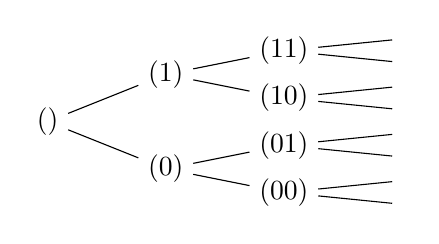
\begin{tikzpicture}
    [
	level 1/.style={sibling distance=12mm},
	level 2/.style={sibling distance=6mm},
	level 3/.style={sibling distance=3mm}
    ]
  \node {()} [grow=right]
    child {node {(0)}
      child {node {(00)} child {node {$\hdots$}} child {node {$\hdots$}}}
      child {node {(01)} child {node {$\hdots$}} child {node {$\hdots$}}}
    }
    child {node {(1)}
      child {node {(10)} child {node {$\hdots$}} child {node {$\hdots$}}}
      child {node {(11)} child {node {$\hdots$}} child {node {$\hdots$}}}
    };
  \end{tikzpicture}
  \end{figure}

  Pour généraliser les types inductifs, on introduit alors les W-types (\textit{well-founded trees}) de Martin-Löf.
  Pour ce faire, on utilise un type $A : \U$ qui correspond aux \textit{étiquettes} et un type $B : A \fun \U$ qui
  permet de coder l'arité des noeuds : un noeud dont l'étiquette est $a : A$ aura une arité de $B(a)$.
  Le type résultant de ces deux types est $W_{a:A} B(a)$ que l'on construit via la règle de formation suivante :

  $$
  \prfinterspace=2em
  \prftree[r]{(W f)}{\Gamma \vdash A : \U}{\Gamma, a : A \vdash B(a) : \U}{\Gamma \vdash W_{a: A} B(a) : \U}
  $$

  Les éléments d'un type $W_{a:A}B(a)$ sont donc des noeuds d'un arbre auxquels on associe la fonction donnant
  les noeuds précédents dans l'arbre. On construit ces éléments à l'aide
  de la règle d'introduction pour les W-types :

  $$
  \prfinterspace=2em
  \prftree[r]{(W i)}{\Gamma \vdash a : A}{\Gamma, a : A \vdash b : B(a) \fun W_{x:A}B(x)}
    {\Gamma \vdash \sup(a, b) : W_{x:A}B(x)}
  $$
  La fonction $\sup$ utilisé dans cette règle est donc de type
  $$\sup : \prod_{a:A}{\left(B(a) \fun W_{x:A}B(x)\right)} \fun W_{a:A}B(a).$$
  Chaque noeud $c :\equiv \sup(a, b) : W_{x:A}B(x)$ est donc relié aux autres par la fonction $b : B(a) \fun W_{x:A}B(x)$,
  en effet si on considère un élément $v : B(a)$ alors $b\ v$ est un prédecesseur du noeud $c$ dans l'arbre $W_{x:A}B(x)$.

  \begin{figure}[ht]
    \centering
    \begin{tikzpicture}
      [
	level 1/.style={sibling distance=25mm},
	level 2/.style={sibling distance=15mm}
      ]
      \node {$\sup(a_1, b_1)$} [grow=down]
	child {node {$b_1\ v_1 = \sup(a_2, b_2)$}
	  child {node {$b_2\ v_2$} edge from parent node[left] {$v_2$}}
	  child {node {$\hdots$}}
	  edge from parent node[left] {$v_1\ $}
	}
	child {node {$\hdots$}}
	child {node {$\hdots$}}
	child [grow=north east] {node {$\hdots$}};
    \end{tikzpicture}
  \end{figure}

  Reprenons l'exemple du type $\N$ des entiers.
  On peut le décrire en terme de W-type en prenant $\N :\equiv W_{x: \textbf{2}}B(x)$ où $B(0_{\textbf{2}}) :\equiv \textbf{0}$
  et $B(1_{\textbf{2}}) :\equiv \textbf{1}$.
  En effet, il y a deux manières de construire un entier : ou bien c'est 0 ou bien il est de la forme $s\ k$ avec $k : \N$.
  Pour 0, son étiquette dans l'arbre est donc $0_{\textbf{2}}$ tandis que les éléments de la forme $s\ k$ ont l'étiquette
  $1_{\textbf{2}}$.
  On peut donc écrire 0 avec la fonction $\sup$ :
  $$ 0 :\equiv \sup(0_{\textbf{2}}, \rec_{\textbf{0}, \N}).$$
  De même la fonction successeur $s : \N \fun \N$ peut être définie de la manière suivante :
  $$ s :\equiv \lambda n.\ \sup(1_{\textbf{2}}, \lambda(x : \textbf{1}).\ n) : \N \fun \N.$$
  Et donc on a $1 :\equiv s\ 0 \equiv \sup(1_{\textbf{2}}, \lambda x.\ 0)$ etc.

  La règle d'élimination décrit le principe d'induction sur les W-types.
  Pour prouver une proposition sur un type inductif, de manière analogue au principe de récurrence des entiers,
  on montre que la proposition est héréditaire, dans le cas présent cela revient à montrer que si la proposition est vraie
  sur tout les sous-arbres, alors elle est vraie sur le noeud reliant ces sous-arbres, c'est ce que dit la dernière prémisse
  de la règle d'élimination, qui s'énonce de la manière suivante :

  $$
  \prfinterspace=2em
  \prftree[r]{(W e)}
  {\Gamma\ \vdash t : W_{x:A}B(x)}
  {
    \prfStackPremises
    % {\Gamma \vdash t : W_{x:A}B(x)}
    {\Gamma, a : A, b : B(a) \fun W_{x:A}B(x),}
    {c : \prod_{v:B(a)}{E(b\ v)}\ \vdash e(a, b, c) : E(\sup(a, b))}
  }
    % {\Gamma, a : A, b : B(a) \fun W_{x:A}B(x), c : \prod_{v : B(a)}{E(f\ v)} \vdash e(a, b, c) : E(\sup(a, b))}
  {\Gamma\ \vdash \rec_{W_{x:A}B(x)}(E, e, t) : E(t)}
  $$
  La fonction $e$ présente dans la règle est de type
  $$e \colon \prod_{a:A}\prod_{b:(B(a) \fun W_{x:A}B(x))}\left(\prod_{v:B(a)}E(b\ v)\right) \fun E(\sup(a, b)).$$
  et pour des éléments $a : A$, $b : B(a) \fun W_{x:A}B(x)$ et une preuve $c$ de $\prod_{v:B(a)}{E(b\ v)}$
  renvoie une preuve de $E(\sup(a, b))$.
  La fonction $\rec_{W_{x:A}B(x)}$ présente dans la conclusion de la règle précédente est une fonction qui à un prédicat
  (ou famille de type) $E$ sur le type $W_{x:A}B(x)$, une fonction $e$ comme décrit juste avant et un élément $t : W_{x:A}B(x)$
  retourne une preuve (ou un élément) de $E(t)$. Ainsi, la fonction $e$ et la fonction $\rec_{W_{x:A}B(x)}$ renvoie des preuves de même nature,
  on peut donc imaginer une relation liant les deux : c'est la règle d'égalité (ou règle de calcul de $\rec_{W_{x:A}B(x)}$).

  $$
  \prfinterspace=2em
  \prftree[r]{(W $\equiv$)}
    {\prfStackPremises
      {\Gamma\ \vdash a : A}
      {\Gamma\ \vdash b : B(a) \fun W_{x:A}B(x)}
      {\Gamma, x : A, x : B(x) \fun W_{x:A}B(x), z : \prod_{v:B(x)}{E(y\ v)}\ \vdash e(x, y, z) : E(\sup(x, y))}
    }
      {\Gamma \vdash \rec_{W_{x:A}B(x)}(E, e, \sup(a, b)) \equiv e(a, b, \lambda v.\ \rec_{W_{x:A}B(x)}(E, e, b\ v)) : E(\sup(a, b))}
  $$

  En effet, pour $a : A$ et $b : B(a) \fun W_{x:A}B(x)$ la fonction $\lambda(v : B(a)).\ \rec_{W_{x:A}B(x)}(E, e, b\ v)$
  retourne une preuve (un élément) de $\prod_{v : B(a)}{E(b \ v)}$, ce qui correspond au
  dernier paramètre de la fonction $e$ et donc le membre de droite de l'égalité est bien une preuve (un élément)
  de $E(\sup(a, b))$ comme voulue.
  Les prémisses de cette règle sont de simple vérifications de typage de $a$, $b$ et $e$.

  \subsubsection{Entiers naturels}

  Avec les W-types, nous pouvons désormais construire les entiers naturels.
  Pour ce faire, on note $\N \equiv W_{x : \2}B(x)$ où $B(0_{\2}) :\equiv \0$ et $B(1_{\2}) :\equiv \1$.
  On a donc déjà vu dans le paragraphe précédent que tout élément de $\N$ s'exprime sous la forme $0$ ou $s\ k$
  avec $k : \N$ et de plus on avait les expressions de $0$ et de $s : \N \fun \N$ suivantes :
  $$\left\{ \begin{array}{rll}
      0 &:\equiv \sup(0_{\2}, \rec_{\0, \N}) 				&: \N \\
      s &:\equiv \lambda(n : \N).\ \sup(1_{\2}, \lambda(x : \1).\ n)	&: \N \fun \N
  \end{array}\right.$$

  On peut également réexprimer les règles de formation, d'introduction, d'élimination et d'égalité dans le cas de $\N$.
  Pour la règle de formation, on obtient :

  $$
  \prfinterspace=2em
  \prftree
    {\prfaxiom{\Gamma\ \vdash \2 : \U}}
    {\prftree
      {\prfaxiom{\Gamma, a : \2\ \vdash B : \2 \fun \U}}
      {\prftree
	{\prfaxiom{\Gamma\ \vdash \2 : \U}}
      {\Gamma, a : \2\ \vdash a : \2}}
    {\Gamma, a : \2\ \vdash B(a) : \U}}
  {\Gamma\ \vdash \N : \U}
  $$

  On a donc la règle simplifiée :

  $$
  \prfbyaxiom{$\N$ i}
    {\Gamma\ \vdash \N : \U}
  $$

  Ensuite, concernant la règle d'introduction on distingue deux cas puisqu'il y a deux manières de construire
  un élément $n : \N$, soit $n \equiv 0$, soit $n \equiv s\ k$ avec $k : \N$.

  $$
  \prfinterspace=2em
  \prftree
    {\prftree
      {\prfaxiom{\Gamma\ \vdash 0_{\2} : \2}}
      {\prftree
	{\prfaxiom{\Gamma, 0_{\2} : \2\ \vdash \rec_{\0, \N} : \0 \fun \N}}
      {\Gamma, 0_{\2} : \2\ \vdash \rec_{\0, \N} : B(0_{\2}) \fun \N}}
    {\Gamma\ \vdash \sup(0_{\2}, \rec_{\0, \N}) : \N}}
  {\Gamma\ \vdash 0 : \N}
  $$

  $$
  \prfinterspace=2em
  \prftree
    {\prfaxiom{\Gamma\ \vdash s : \N \fun \N}}
    {\Gamma\ \vdash k : \N}
  {\Gamma \vdash s\ k : \N}
  $$
  Ce qui donne les deux règles d'introduction de $\N$ :
  $$\begin{array}{cc}
    \prfbyaxiom{($0$ i)}{\Gamma\ \vdash 0 : \N}\hspace{2cm} & \prftree[r]{($s$ i)}{\Gamma\ \vdash k : \N}{\Gamma\ \vdash s\ k : \N}
  \end{array}$$

  Pour la règle d'élimination sur le type $\N$, on s'attend à retrouver le principe de récurrence usuel sur les entiers,
  à savoir que si une prédicat $E : \N \fun \U$ est vrai sur $0$ et que si $E(k)$ est vrai alors $E(s\ k)$ est vrai,
  alors $E(k)$ est vrai sur tout $k : \N$.
  $$
  \prfinterspace=1.2em
  \prftree
    {\Gamma\ \vdash k : \N}
    {\prftree
      {\text{Lemme 1}}
      {\text{Lemme 2}}
    {\Gamma, a : \2, b : B(a) \fun \N, c : \prod_{v : B(a)}{E(b\ v)}\ \vdash e(a, b, c) : E(\sup(a, b))}}
    {\Gamma\ \vdash \rec_{\N}(E, e, k) : E(k)}
  $$
  Avec
  $$\prfinterspace=1.2em
  \prftree[r]{Lemme 1}
    {\Gamma, a : \1, b : \0 \fun \N, c : \prod_{v : \0}E(b\ v) \vdash e(a, b, c) : E(\sup(0_{\2}, b))}
  {\Gamma, a : \1, b : B(\inl(a)) \fun \N, c : \prod_{v : B(\inl(a))}E(b\ v) \vdash e(a, b, c) : E(\sup(a, b))}
  $$
  et
  $$\prfinterspace=1.2em
  \prftree[r]{Lemme 2}
  {\Gamma, a : \1, b : \1 \fun \N, c : \prod_{v : \1}E(b\ v) \vdash e(a, b, c) : E(\sup(1_{\2}, b))}
  {\Gamma, a : \1, b : B(\inr(a)) \fun \N, c : \prod_{v:B(\inr(a))}E(b\ v) \vdash e(a, b, c) : E(\sup(\inr(a), b))}
  $$
  On peut simplifier les prémisses du Lemme 1 en remaquant que ses hypothèses sont triviales et que $\sup(0_{\2}, b) \equiv 0$
  pour toute fonction $b : \0 \fun \N$, ce qui donne après simplification :
  $$\Gamma \vdash e_0 : E(0).$$
  De même, pour le Lemme 2 en remaquant qu'un fonction $b : \1 \fun \N$ est équivalent à choisir un $k : \N$ et que
  $c : \prod_{v:\1}E(b\ v)$ est similaire à $c : E(k)$, on peut réécrire la prémisse en
  $$\Gamma, k : \N, p : E(k) \vdash e_s(k, p) : E(s\ k).$$
  Finalement, on peut décomposer la fonction $e$ du recurseur : $e_0 : E(0)$ et $e_s : \prod_{k : \N}E(k) \fun E(s\ k)$,
  ce qui permet de réécrire la règle d'élimination sous la forme plus simple :

  $$\prfinterspace=1.2em
  \prftree[r]{$\N$ e}
    {\Gamma \vdash k : \N}
    {\Gamma \vdash e_0 : E(0)}
    {\Gamma, k : \N, p : E(k) \vdash e_s(k, p) : E(s\ k)}
  {\Gamma \vdash \rec_{\N}(E, e_0, e_s, k) : E(k)}
  $$
  On retrouve bien le principe de récurrence usuel, en effet pour prouver un prédicat sur les entiers $\N$
  il suffit de le prouver sur $0$ puis qu'il est héréditaire \textit{ie}. s'il est vérifié sur un entier $k : \N$
  alors il est vérifié sur $s\ k$ l'entier suivant.

  \subsubsection{Listes}

  Un autre exemple de type inductif est le type des listes sur un type $A : \U_i$, que l'on note $L(A)$.
  Pour la construire on utilise alors le W-type $W_{x:\1+A}B(x)$ où $B(\inl(\star)) \equiv \0$ et $B(\inr(a)) \equiv \1$,
  autrement dit on pose
  $$L(A) \equiv W_{x:\1 + A}\rec_{1+A}(\U_i, \lambda(x : \1).\ \0, \lambda(a : A).\ \1, x).$$
  De là, on déduit la règle de formation de $L(A)$ :
  $$
  \prfinterspace=1.2em
  \prftree
    {
      \prftree
	{\Gamma \vdash A : \U_i}
	{\prftree{\Gamma \ctx}{\Gamma \vdash \1 : \U_i}}
	  {\Gamma \vdash \1 + A : \U_i}
    }
    {
      \prftree
	{\prfaxiom{\Gamma, x : \1 + A \vdash \rec_{\1+A}(\U_i, \lambda(y : \1).\ \0, \lambda(y : A).\ \1, x) : \U_i}}
	{\Gamma, x : \1 + A \vdash B(x) : \U_i}
    }
      {\Gamma \vdash L(A) : \U_i}
  $$
  Plus simplement,
  $$
  \prftree[r]{$L$ f}{\Gamma \vdash A : \U_i}{\Gamma \vdash L(A) : \U_i}
  $$

  Ensuite pour construire un élément on a deux constructeurs :
  \begin{itemize}
    \item La liste vide, notée $()$ que l'on définit comme $() :\equiv \sup(\inl(\star), \rec_{\0}(L(A))) : L(A)$,
    \item L'ajout d'un élément en tête de liste via la fonction $c : A \fun L(A) \fun L(A)$ qui est définit de la manière suivante :
      $$c :\equiv \lambda(a : A).\ \lambda(l : L(A)).\ \sup(a, \lambda(x : \1).\ l).$$
      que l'on peut également noter $::$ de manière infixe.
  \end{itemize}
  Ainsi, une liste $l \equiv (a_1, \hdots, a_k) : L(A)$ est définie par
  $$l :\equiv c\ a_1\ (a_2, \hdots, a_k) \equiv a_1 :: (a_2, \hdots, a_k) \equiv \sup(a_1, \lambda(x : \1).\ (a_2, \hdots, a_k)).$$
  On remarque alors une structure d'arbre dans le type des listes, dont la racine est $()$
  et la fonction donnant les successeurs d'un noeud $l$ est la fonction $\lambda(a:A).\ c\ a\ l : A \fun L(A)$.

  On a donc deux règles d'introduction correspondant à ces deux cas.

  $$
  \prfinterspace=1.2em
  \prftree
    {\prftree
      {\prftree
	{\prfaxiom{\Gamma \vdash \1 : \U_i}}
	{\Gamma \vdash A : \U_i}
	{\prfaxiom{\Gamma \vdash \star : \1}}
      {\Gamma \vdash \inl(\star) : \1 + A}}
      {\prftree
	{\prfaxiom{\Gamma \vdash \rec_{\0}(L(A)) : \0 \fun L(A)}}
      {\Gamma\vdash \rec_{\0}(L(A)) : B(\inl(\star)) \fun L(A)}}
    {\Gamma \vdash \sup(\inl(\star), \rec_{\0}(L(A))) : L(A)}}
  {\Gamma \vdash () : L(A)}
  $$

  $$
    \prfinterspace=1.2em
    \prftree
      {\prftree
	{\prftree
	  {\prfaxiom{\Gamma \vdash \1 : \U_i}}
	  {\Gamma \vdash A : \U_i}
	  {\Gamma \vdash a : A}
	{\Gamma \vdash \inr(a) : \1 + A}}
	{\prftree
	  {\prftree
	    {\prftree
	      {\prftree
		{\Gamma \vdash l : L(A)}
	      {\Gamma, x : \1 \vdash l : L(A)}}
	    {\Gamma \vdash \lambda(x:\1).\ l : \1 \fun L(A)}}
	  {\Gamma \vdash \lambda(x:\1).\ l : \rec_{\1 + A}(\U_i, \0, \1, \inr(a)) \fun L(A)}}
	{\Gamma \vdash \lambda(x:\1).\ l : B(\inr(a)) \fun L(A)}}
      {\Gamma \vdash \sup(\inr(a), \lambda(x:\1).\ l) : L(A)}}
    {\Gamma \vdash a :: l : L(A)}
  $$
  Plus simplement,

  $$\prfinterspace=1.2em
  \begin{array}{cc}
    \prftree[r]{$()$ i}{\Gamma \vdash A : \U_i}{\Gamma \vdash () : L(A)} \hspace{1cm}
    & \prftree[r]{$c$ i}{\Gamma \vdash A : \U_i}{\Gamma \vdash a : A}{\Gamma \vdash l : L(A)}{\Gamma \vdash a :: l : L(A)}
  \end{array}$$

  A partir de la règle d'élimination des W-types, on peut déduire la règle d'élimination du type $L(A)$ :

  $$\prfinterspace=1.2em
  \prftree
    {\Gamma \vdash l : L(A)}
    {\prftree
      {\text{Lemme 1}}
      {\text{Lemme 2}}
    {\Gamma, a : \1 + A, b : B(a) \fun L(A), c : \prod_{v:B(a)}E(b\ v) \vdash e(a, b, c) : E(\sup(a, b))}}
  {\Gamma \vdash \rec_{L(A)}(E, e, l) : E(l)}
  \vspace{1em}
  $$
  $$\prfinterspace=1.2em
  \prftree[r]{Lemme 1}
    {\Gamma, a : \1, b : \0 \fun L(A), c : \prod_{v:\0}E(b\ v) \vdash e(a, b, c) : E(())}
  {\Gamma, a : \1, b : B(\inl(a)) \fun L(A), c : \prod_{v:B(\inl(a))}E(b\ v) \vdash e(a, b, c) : E(\sup(\inl(a), b))}
  \vspace{1em}
  $$
  $$\prfinterspace=1.2em
  \prftree[r]{Lemme 2}
    {\Gamma, a : A, b : \1 \fun L(A), c : \prod_{v: \1}E(b\ v) \vdash e(a, b, c) : E(a :: b)}
  {\Gamma, a : A, b : B(\inr(a)) \fun L(A), c : \prod_{v:B(\inr(a))}E(b\ v) \vdash e(a, b, c) : E(\sup(\inr(a), b))}
  $$
  Le lemme 1 correspond à une preuve de $E$ sur la liste vide $()$ dont les hypothèses sont triviales.
  On peut donc réécrire sa prémisse sous une forme plus simple
  $$\Gamma \vdash e_0 : E(()).$$
  De même, on peut simplifier le lemme 2 en remarquant que $b : \1 \fun L(A)$ est équivalent à une liste $l \equiv b\ \star$,
  et que $c : \prod_{v:\1}E(b\ v)$ est une preuve de $E(l)$ :
  $$\Gamma, a : A, l : L(A), p : E(l) \vdash e_s(a, l, p) : E(a :: l).$$
  On peut aussi réécrire $e$ en le décomposant en $e_0 : E(())$ et $e_s : \prod_{a:A}\prod_{l:L(A)}E(l)$
  pour correspondre à ces deux cas, ce qui donne finalement la règle
  $$
  \prfinterspace=1.2em
  \prftree[r]{$L$ e}
    {\Gamma \vdash l : L(A)}
    {\Gamma \vdash e_0 : E(())}
    {\Gamma, a : A, l : L(A), p : E(l) \vdash e_s(a, l, p) : E(a :: l)}
  {\Gamma \vdash \rec_{L(A)}(E, e_0, e_s, l) : E(l)}
  $$
  Ce qui correspond à la preuve par induction sur les listes, à savoir que si un prédicat $E$ sur $L(A)$ est vraie
  sur la liste vide $()$ et qu'il est héréditaire \textit{ie.} si $E$ est vraie sur une liste $l$ et si $a : A$
  alors $E$ est vérifié sur $a :: l$, alors $E$ est vérifié sur toute les listes.

  \subsubsection{Produit}

  \subsubsection{Paires dépendantes ($\Sigma$-type)}

\end{document}
